% Options for packages loaded elsewhere
\PassOptionsToPackage{unicode}{hyperref}
\PassOptionsToPackage{hyphens}{url}
%
\documentclass[
]{article}
\usepackage{amsmath,amssymb}
\usepackage{lmodern}
\usepackage{iftex}
\ifPDFTeX
  \usepackage[T1]{fontenc}
  \usepackage[utf8]{inputenc}
  \usepackage{textcomp} % provide euro and other symbols
\else % if luatex or xetex
  \usepackage{unicode-math}
  \defaultfontfeatures{Scale=MatchLowercase}
  \defaultfontfeatures[\rmfamily]{Ligatures=TeX,Scale=1}
\fi
% Use upquote if available, for straight quotes in verbatim environments
\IfFileExists{upquote.sty}{\usepackage{upquote}}{}
\IfFileExists{microtype.sty}{% use microtype if available
  \usepackage[]{microtype}
  \UseMicrotypeSet[protrusion]{basicmath} % disable protrusion for tt fonts
}{}
\makeatletter
\@ifundefined{KOMAClassName}{% if non-KOMA class
  \IfFileExists{parskip.sty}{%
    \usepackage{parskip}
  }{% else
    \setlength{\parindent}{0pt}
    \setlength{\parskip}{6pt plus 2pt minus 1pt}}
}{% if KOMA class
  \KOMAoptions{parskip=half}}
\makeatother
\usepackage{xcolor}
\IfFileExists{xurl.sty}{\usepackage{xurl}}{} % add URL line breaks if available
\IfFileExists{bookmark.sty}{\usepackage{bookmark}}{\usepackage{hyperref}}
\hypersetup{
  hidelinks,
  pdfcreator={LaTeX via pandoc}}
\urlstyle{same} % disable monospaced font for URLs
\usepackage[margin=1in]{geometry}
\usepackage{graphicx}
\makeatletter
\def\maxwidth{\ifdim\Gin@nat@width>\linewidth\linewidth\else\Gin@nat@width\fi}
\def\maxheight{\ifdim\Gin@nat@height>\textheight\textheight\else\Gin@nat@height\fi}
\makeatother
% Scale images if necessary, so that they will not overflow the page
% margins by default, and it is still possible to overwrite the defaults
% using explicit options in \includegraphics[width, height, ...]{}
\setkeys{Gin}{width=\maxwidth,height=\maxheight,keepaspectratio}
% Set default figure placement to htbp
\makeatletter
\def\fps@figure{htbp}
\makeatother
\setlength{\emergencystretch}{3em} % prevent overfull lines
\providecommand{\tightlist}{%
  \setlength{\itemsep}{0pt}\setlength{\parskip}{0pt}}
\setcounter{secnumdepth}{-\maxdimen} % remove section numbering
\newlength{\cslhangindent}
\setlength{\cslhangindent}{1.5em}
\newlength{\csllabelwidth}
\setlength{\csllabelwidth}{3em}
\newlength{\cslentryspacingunit} % times entry-spacing
\setlength{\cslentryspacingunit}{\parskip}
\newenvironment{CSLReferences}[2] % #1 hanging-ident, #2 entry spacing
 {% don't indent paragraphs
  \setlength{\parindent}{0pt}
  % turn on hanging indent if param 1 is 1
  \ifodd #1
  \let\oldpar\par
  \def\par{\hangindent=\cslhangindent\oldpar}
  \fi
  % set entry spacing
  \setlength{\parskip}{#2\cslentryspacingunit}
 }%
 {}
\usepackage{calc}
\newcommand{\CSLBlock}[1]{#1\hfill\break}
\newcommand{\CSLLeftMargin}[1]{\parbox[t]{\csllabelwidth}{#1}}
\newcommand{\CSLRightInline}[1]{\parbox[t]{\linewidth - \csllabelwidth}{#1}\break}
\newcommand{\CSLIndent}[1]{\hspace{\cslhangindent}#1}
\usepackage{booktabs}
\usepackage{longtable}
\usepackage{array}
\usepackage{multirow}
\usepackage{wrapfig}
\usepackage{float}
\usepackage{colortbl}
\usepackage{pdflscape}
\usepackage{tabu}
\usepackage{threeparttable}
\usepackage{threeparttablex}
\usepackage[normalem]{ulem}
\usepackage{makecell}
\usepackage{xcolor}
\ifLuaTeX
  \usepackage{selnolig}  % disable illegal ligatures
\fi

\author{}
\date{\vspace{-2.5em}}

\begin{document}

{
\setcounter{tocdepth}{2}
\tableofcontents
}
\newpage

LMA responses of understory plants to artificial light at night

\[ \]

Cong Zhou\textsuperscript{1,2}, Masatoshi Katabuchi\textsuperscript{1},
Akihiro Nakamura\textsuperscript{1},

\[ \]

\textsuperscript{1} CAS Key Laboratory of Tropical Forest Ecology,
Xishuangbanna Tropical Botanical Garden, Chinese Academy of Sciences,
Menglun, Yunnan 666303, China

\textsuperscript{2} University of Chinese Academy of Sciences, Beijing
100049, China

\[ \]

\textbf{Corresponding Authors}:

Masatoshi Katabuchi

E-mail:
\href{mailto:mattocci27@gmail.com}{\nolinkurl{mattocci27@gmail.com}}

\[ \]

Manuscript received \_\_\_\_\_\_\_; revision accepted \_\_\_\_\_\_\_.

\textbf{Running title}:

\newpage

\hypertarget{abstract}{%
\section{ABSTRACT}\label{abstract}}

\textbf{PREMISE:}

\textbf{METHODS:}

\textbf{RESULTS:}

\textbf{CONCLUSIONS:}

\textbf{KEY WORDS} light pollution, leaf mass per area(LMA), leaf punch,
Artificial light at night(ALAN),

\hypertarget{introduction}{%
\section{INTRODUCTION}\label{introduction}}

Artificial light at night(ALAN), consists of artificial light sources
emission and the light reflected back from the sky(skyglow), had
disturbed ecological processes since the start of 20th century
(\protect\hyperlink{ref-Bennie2016}{Bennie et al. 2016};
\protect\hyperlink{ref-Longcore2004}{Longcore and Rich 2004};
\protect\hyperlink{ref-Gaston2013}{Gaston et al. 2013}). So far,
artificial light at night extends both in intensity covered a large
illuminance range from the degree hard to detect to almost daylight and
in extent covered more and more World's terrestrial surfaces
(\protect\hyperlink{ref-Bennie2016}{Bennie et al. 2016};
\protect\hyperlink{ref-Falchi2016}{2016}). Oganisms as well as habitats
could be effected directly near artificial light at night(ALAN) such as
streetlight and indirectly by sky glow scattered from city ALAN at
rural-urban continuum. Ignoring the effect of artificial light at night
to multilevel ecological processes is self-deception, hence more and
more research would be carried through about this important
topic(\protect\hyperlink{ref-Davies2018}{Davies and Smyth 2018}).

Artificial light at night calls effects among wild taxonomic groups both
zoology and botany, from mammals, birds, reptiles and amphibians,
fishes, invertebrates and plants
etc(\protect\hyperlink{ref-Rich2006}{Rich and Longcore 2006}).
Typically, lighted towers and glow of city lights confuse migrating
birds(\protect\hyperlink{ref-Loss2014}{Loss et al. 2014}), and
streetlight attracting sea turtle hatchlings which dead
parched(\protect\hyperlink{ref-Brei2016}{Brei, Pérez-Barahona, and
Strobl 2016}). Recently study shows ALAN is an important bringer to
drive insects population decline
(\protect\hyperlink{ref-Boyes2021}{Boyes et al. 2021};
\protect\hyperlink{ref-Owens2020}{Owens et al. 2020}). And to plants,
biomass would increase responsing to ALAN and show different ratio
between widely and less‐widely naturalized alien
plants(\protect\hyperlink{ref-Speiuxdfer2021}{\textbf{Speißer2021?}}).
Generally, artificial light at night could cause ecological effects
spanning trophic levels, and the impacts depends on the
wavelengths(\protect\hyperlink{ref-Bennie2018}{Bennie et al. 2018}).
However, no rigorous studies have examined effects of artificial light
at night on plants in conditions close to their natural environment.

In previous study, it has been demonstrated that nitrogen contents per
unit leaf area \(N_a\) increased with environmental nitrogen contents,
while LMA shows different correlation decreasing with N supply
(\protect\hyperlink{ref-Jullien2009}{Jullien et al. 2009};
\protect\hyperlink{ref-An2008}{An and Shangguan 2008}). Wright
(\protect\hyperlink{ref-Wright2019}{2019}) shows nutrients clearly limit
tropical forest plants, and especially the limitation of N and P in both
lowland and montane forests. Hence, besides the direct effect from ALAN
the nutrients condition of the plants should also jump into our sight.
By the light compass theory (\protect\hyperlink{ref-Baker1978}{Baker and
Sadovy 1978}; \protect\hyperlink{ref-Sotthibandhu1979}{Sotthibandhu and
Baker 1979}) that insects orient themselves by maintaining a constant
angle to light rays, artificial light at night plays a role of sink
attracting insects which replaces the role of the moon and stars to a
great extent. Further more, it's been showed that about 30\%--40\% of
insects die soon thereafter approaching street lamps for collision,
overheating, dehydration, or predation
(\protect\hyperlink{ref-Minnaar2015}{Minnaar et al. 2015};
\protect\hyperlink{ref-Owens2018}{Owens and Lewis 2018}). Then comes our
research hypothesis that ALAN would decrease LMA of plants around it
indirectly as a side-effect of gathering phototaxis insects which
chagnes the nutrients condition by distance.

Although LMA driven by inherent genetic
mechanisms(\protect\hyperlink{ref-Asner2011}{Asner et al. 2011}),
environmental stresses (temperature, water and light) also shapes LMA.
Acually, plants could sense light through photorecpetors which allows
the plant to respond to four parameters of their light environment:
light spectral quality, light intensity, light direction, and light
duration(\protect\hyperlink{ref-Paik2019}{Paik and Huq 2019};
\protect\hyperlink{ref-Rich2006}{Rich and Longcore 2006}). For
individual species, LMA was proportional with species distributions
along the insolation gradient, and was significantly higher in evergreen
versus deciduous species(\protect\hyperlink{ref-Ackerly2002}{Ackerly et
al. 2002}; \protect\hyperlink{ref-Onoda2008}{Onoda, Schieving, and Anten
2008}; \protect\hyperlink{ref-Niinemets2004}{Niinemets, Kull, and
Tenhunen 2004}). Here, ALAN could be considered as a conduct of
prolonging light duration to plants so plants LMA could increase with
that.

To know the effets of artificial light at night on perfomance of
understory species so as a simulation to the city street shrubs, we
conducted a forest artificial light experiment. Two species were chosen
in this experiment representing sun species and shade species
respectively to test whether different responds would show between them.
We predicted that artificial light at night would bring effect to
understory both aboveground as direct light supplementary and undergound
as indirect soil nutrients supplementary. And we also predicted that
canopy-openness and its interaction with artificial light at night would
show weaker impaction in this experiment.

\hypertarget{materials-and-methods}{%
\section{MATERIALS AND METHODS}\label{materials-and-methods}}

\emph{experimental setup}

The field experiment was located within the Xishuangbanna Tropical
Botanical Garden(XTBG),China in rubber tree forest(N21°54' E101°16')
where we totally set 5 plots and selected 2 plots for this this after
field investiation. LED (10w) is used to create an artificial light
environment in all plots at night. The LED system includes 6 components.
A metal box with an opening is used as a rainproof protector which is
attached to a tree at around 1.2 m from the ground. A rechargeable
lithium battery (12v/30Ah) and an electric timer controls the timing and
duration of the LED light operation at night. An electric wire was used
to connect battery and LED which was hanging from a tree branch with a
lampshade at approximately 2 m from the ground. Then the LED would work
automatically from 8 pm to 5 am every day. This experiment started from
2019 November, and samples were collected on 2021 November.

\emph{Species Selection}

Considering the understory condition (enough mature individual numbers,
distribution of individuals) and species specificity(it should be
evergreen species, and not be the nitrogen fix plants like Leguminosae)
of each plot, finally two species respectively in two plots were chosen
for our study, \emph{Colocasia gigantea (Blume) Hook. f.} representing
shade species and \emph{Melastoma candidum D. Don} for sun species.

\emph{Measurements}

We measured the horizontal distance and geographic orientation of each
individual away from the LED using tape measure representing the
relative effects of ALAN. Canopy openness was selected to be on behalf
of day light, which photographed by Nikon COOLPIX4500 with fish-eye
lens(Nikon FC-e8) then measured using R package
\emph{LeafArea}(\protect\hyperlink{ref-Katabuchi2015}{Katabuchi 2015}).
For leaf mass per area(LMA), we use leaf disc(10mm\^{}2) punched from
leaf avoiding vein and leaf margin instead of whole-leaf to calculate
LMA value.

\emph{Data Analysis}

To analyze the effects of ALAN, daylight's effect, and their interaction
on both \emph{Melastoma candidum D. Don} and \emph{Colocasia gigantea
(Blume) Hook. f.}, We fitted a Bayesian linear mixed-effets model for
each species using `rstan' package in R. Leaf mass per area(LMA) of each
leaf of each individual was the response variable. Distance from the
ALAN of each individual was transformed by log and reciprocal for both
the accumulation of insects and the intensity of ALAN fade away from
distance. We conducted individual as a random effect for each species on
our model, for the non-independence of individuals of the same species.
All statistical analyses were conducted in R version 4.1.2
(\protect\hyperlink{ref-RCoreTeam2021}{\textbf{RCoreTeam2021?}}). ** how
to cite R? **

\hypertarget{results}{%
\section{RESULTS}\label{results}}

For species \emph{Colocasia gigantea (Blume) Hook. f.}, both the effcts
of ALAN and daylight were significant, while species \emph{Melastoma
candidum D. Don} showed no significance. Artificial light at night drove
the averaged individual LMA value decrease for species \emph{Colocasia
gigantea (Blume) Hook. f.} (mean: -0.1043) and for species
\emph{Melastoma candidum D. Don} (mean: -0.0422) although not
significant. Both species showed no significance on the interaction of
the effects of ALAN and daylight. (Table 1.)

\hypertarget{discussion}{%
\section{DISCUSSION}\label{discussion}}

Although it has been demonstrated that LMA increase with
insolation{[}{]}, our research shows the artificial light situation
could make differences. Actually, artificial light at night exerts an
influence on the physiological processes of understory by multi-approach
both aboveground and undergound. For aboveground part, artificial light
at night change the light environments of plants including light
duration, light intensity and light spectral quality. For underground
part, artificial light at night indirectly changed the soil nutrients
conditions especially as an important nitrogen supplementary. So the
response results of understory could vary according to the species
specificity{[}{]} and artificial light resource{[}{]}.

There was research showed that plants' biomass would increase under
artificial light{[}{]}, our study showed the change part of biomass
could be channelled into mixed results. Further more, adequate tests of
the influence of artificial light at night on understory will entail
more experimental work under field conditions. Controlling experiment
probably tend to underestimate the environmental heterogeneity and
species interaction, because many irreplaceable features of field
conditions, such as subtle nutrients change, herbivores and competitors
are usually absent. Hence the general pattern how understory species
responds to artificial light at night remains unknown. In future work,
diverse artificial light resource in light spectral quality and light
intensity is need to simulate multi-situation of artificial light. And
if possible, long term field experiment combining with controlling
experiment approaching to plants natural growth situation will figure
out the generalized patterns.

In conclusion, our study showed the LMA of some understory species would
decrease with artificial light at night. The effects of artificial light
at night consists of aboveground part directly as light resource and
undergound part indirectly as soil nutrients. Still, more studies are
needed to reveal the comprehensive effcts, from plant physiology to
plant community. Nevertheless, the negative effct of artificial light at
night on understory species indicates that increments of artificial
light at night might bring about a physiological suppression to those
understory plants.

\hypertarget{ackonwlegements}{%
\section{ACKONWLEGEMENTS}\label{ackonwlegements}}

\hypertarget{author-contributions}{%
\section{AUTHOR CONTRIBUTIONS}\label{author-contributions}}

MK and CZ conceived the study; CZ collected data and performed the
analysis with MK together; all authors contributed to revisions.

\hypertarget{data-availability-statement}{%
\section{DATA AVAILABILITY
STATEMENT}\label{data-availability-statement}}

\hypertarget{supporting-information}{%
\section{SUPPORTING INFORMATION}\label{supporting-information}}

\hypertarget{literature-cited}{%
\section{LITERATURE CITED}\label{literature-cited}}

\hypertarget{refs}{}
\begin{CSLReferences}{1}{0}
\leavevmode\vadjust pre{\hypertarget{ref-Ackerly2002}{}}%
Ackerly, D., C. Knight, S. Weiss, K. Barton, and K. Starmer. 2002.
{``Leaf Size, Specific Leaf Area and Microhabitat Distribution of
Chaparral Woody Plants: Contrasting Patterns in Species Level and
Community Level Analyses.''} \emph{Oecologia} 130 (3): 449--57.
\url{https://doi.org/10.1007/s004420100805}.

\leavevmode\vadjust pre{\hypertarget{ref-An2008}{}}%
An, H., and Z. P. Shangguan. 2008. {``Specific Leaf Area, Leaf Nitrogen
Content, and Photosynthetic Acclimation of {Trifolium} Repens {L}.
Seedlings Grown at Different Irradiances and Nitrogen Concentrations.''}
\emph{Photosynthetica} 46 (1).
\url{https://doi.org/10.1007/s11099-008-0023-y}.

\leavevmode\vadjust pre{\hypertarget{ref-Asner2011}{}}%
Asner, Gregory P., Roberta E. Martin, Raul Tupayachi, Ruth Emerson,
Paola Martinez, Felipe Sinca, George V. N. Powell, S. Joseph Wright, and
Ariel E. Lugo. 2011. {``Taxonomy and Remote Sensing of Leaf Mass Per
Area ({LMA}) in Humid Tropical Forests.''} \emph{Ecological
Applications} 21 (1): 85--98. \url{https://doi.org/10.1890/09-1999.1}.

\leavevmode\vadjust pre{\hypertarget{ref-Baker1978}{}}%
Baker, R. Robin, and Yvonne Sadovy. 1978. {``The Distance and Nature of
the Light-Trap Response of Moths.''} \emph{Nature} 276 (December):
818--21. \url{https://doi.org/10.1038/276818a0}.

\leavevmode\vadjust pre{\hypertarget{ref-Bennie2018}{}}%
Bennie, Jonathan, Thomas W. Davies, David Cruse, Fraser Bell, and Kevin
J. Gaston. 2018. {``Artificial Light at Night Alters Grassland
Vegetation Species Composition and Phenology.''} \emph{Journal of
Applied Ecology} 55 (1): 442--50.
\url{https://doi.org/10.1111/1365-2664.12927}.

\leavevmode\vadjust pre{\hypertarget{ref-Bennie2016}{}}%
Bennie, Jonathan, Thomas W. Davies, David Cruse, and Kevin J. Gaston.
2016. {``Ecological Effects of Artificial Light at Night on Wild
Plants.''} \emph{Journal of Ecology} 104 (3): 611--20.
\url{https://doi.org/10.1111/1365-2745.12551}.

\leavevmode\vadjust pre{\hypertarget{ref-Boyes2021}{}}%
Boyes, Douglas H., Darren M. Evans, Richard Fox, Mark S. Parsons, and
Michael J. O. Pocock. 2021. {``Street Lighting Has Detrimental Impacts
on Local Insect Populations.''} \emph{Science Advances} 7 (35):
eabi8322. \url{https://doi.org/10.1126/sciadv.abi8322}.

\leavevmode\vadjust pre{\hypertarget{ref-Brei2016}{}}%
Brei, Michael, Agustín Pérez-Barahona, and Eric Strobl. 2016.
{``Environmental Pollution and Biodiversity: {Light} Pollution and Sea
Turtles in the {Caribbean}.''} \emph{Journal of Environmental Economics
and Management} 77 (May): 95--116.
\url{https://doi.org/10.1016/j.jeem.2016.02.003}.

\leavevmode\vadjust pre{\hypertarget{ref-Davies2018}{}}%
Davies, Thomas W., and Tim Smyth. 2018. {``Why Artificial Light at Night
Should Be a Focus for Global Change Research in the 21st Century.''}
\emph{Global Change Biology} 24 (3): 872--82.
\url{https://doi.org/10.1111/gcb.13927}.

\leavevmode\vadjust pre{\hypertarget{ref-Falchi2016}{}}%
Falchi. 2016. {``The New World Atlas of Artificial Night Sky
Brightness.''} https://www.science.org/doi/10.1126/sciadv.1600377.
\url{https://doi.org/10.1126/sciadv.1600377}.

\leavevmode\vadjust pre{\hypertarget{ref-Gaston2013}{}}%
Gaston, Kevin J., Jonathan Bennie, Thomas W. Davies, and John Hopkins.
2013. {``The Ecological Impacts of Nighttime Light Pollution: A
Mechanistic Appraisal.''} \emph{Biological Reviews} 88 (4): 912--27.
\url{https://doi.org/10.1111/brv.12036}.

\leavevmode\vadjust pre{\hypertarget{ref-Jullien2009}{}}%
Jullien, Alexandra, Jean-Michel Allirand, Amélie Mathieu, Bruno Andrieu,
and Bertrand Ney. 2009. {``Variations in Leaf Mass Per Area According to
{N} Nutrition, Plant Age, and Leaf Position Reflect Ontogenetic
Plasticity in Winter Oilseed Rape ({Brassica} Napus {L}.).''}
\emph{Field Crops Research} 114 (2): 188--97.
\url{https://doi.org/10.1016/j.fcr.2009.07.015}.

\leavevmode\vadjust pre{\hypertarget{ref-Katabuchi2015}{}}%
Katabuchi, Masatoshi. 2015. {``{LeafArea}: An {R} Package for Rapid
Digital Image Analysis of Leaf Area.''} \emph{Ecological Research} 30
(6): 1073--77. \url{https://doi.org/10.1007/s11284-015-1307-x}.

\leavevmode\vadjust pre{\hypertarget{ref-Longcore2004}{}}%
Longcore, Travis, and Catherine Rich. 2004. {``Ecological Light
Pollution.''} \emph{Frontiers in Ecology and the Environment} 2 (4):
191--98.
\url{https://doi.org/10.1890/1540-9295(2004)002\%5B0191:ELP\%5D2.0.CO;2}.

\leavevmode\vadjust pre{\hypertarget{ref-Loss2014}{}}%
Loss, Scott R., Tom Will, Sara S. Loss, and Peter P. Marra. 2014.
{``Bird\textendash building Collisions in the {United States}:
{Estimates} of Annual Mortality and Species Vulnerability.''} \emph{The
Condor} 116 (1): 8--23. \url{https://doi.org/10.1650/CONDOR-13-090.1}.

\leavevmode\vadjust pre{\hypertarget{ref-Minnaar2015}{}}%
Minnaar, Corneile, Justin G. Boyles, Ingrid A. Minnaar, Catherine L.
Sole, and Andrew E. McKechnie. 2015. {``Stacking the Odds: Light
Pollution May Shift the Balance in an Ancient Predator\textendash prey
Arms Race.''} \emph{Journal of Applied Ecology} 52 (2): 522--31.
\url{https://doi.org/10.1111/1365-2664.12381}.

\leavevmode\vadjust pre{\hypertarget{ref-Niinemets2004}{}}%
Niinemets, Ü., O. Kull, and J. D. Tenhunen. 2004. {``Within-Canopy
Variation in the Rate of Development of Photosynthetic Capacity Is
Proportional to Integrated Quantum Flux Density in Temperate Deciduous
Trees.''} \emph{Plant, Cell \& Environment} 27 (3): 293--313.
\url{https://doi.org/10.1111/j.1365-3040.2003.01143.x}.

\leavevmode\vadjust pre{\hypertarget{ref-Onoda2008}{}}%
Onoda, Y., F. Schieving, and N. P. R. Anten. 2008. {``Effects of {Light}
and {Nutrient Availability} on {Leaf Mechanical Properties} of
{Plantago} Major: {A Conceptual Approach}.''} \emph{Annals of Botany}
101 (5): 727--36. \url{https://doi.org/10.1093/aob/mcn013}.

\leavevmode\vadjust pre{\hypertarget{ref-Owens2020}{}}%
Owens, Avalon C. S., Précillia Cochard, Joanna Durrant, Bridgette
Farnworth, Elizabeth K. Perkin, and Brett Seymoure. 2020. {``Light
Pollution Is a Driver of Insect Declines.''} \emph{Biological
Conservation} 241 (January): 108259.
\url{https://doi.org/10.1016/j.biocon.2019.108259}.

\leavevmode\vadjust pre{\hypertarget{ref-Owens2018}{}}%
Owens, Avalon C. S., and Sara M. Lewis. 2018. {``The Impact of
Artificial Light at Night on Nocturnal Insects: {A} Review and
Synthesis.''} \emph{Ecology and Evolution} 8 (22): 11337--58.
\url{https://doi.org/10.1002/ece3.4557}.

\leavevmode\vadjust pre{\hypertarget{ref-Paik2019}{}}%
Paik, Inyup, and Enamul Huq. 2019. {``Plant Photoreceptors:
{Multi-functional} Sensory Proteins and Their Signaling Networks.''}
\emph{Seminars in Cell \& Developmental Biology} 92 (August): 114--21.
\url{https://doi.org/10.1016/j.semcdb.2019.03.007}.

\leavevmode\vadjust pre{\hypertarget{ref-Rich2006}{}}%
Rich, Catherine, and Travis Longcore. 2006. {``Ecological Consequences
of Artificial Night Lighting.''} In.

\leavevmode\vadjust pre{\hypertarget{ref-Sotthibandhu1979}{}}%
Sotthibandhu, S., and R. R. Baker. 1979. {``Celestial Orientation by the
Large Yellow Underwing Moth, {Noctua} Pronuba {L}.''} \emph{Animal
Behaviour} 27 (August): 786--800.
\url{https://doi.org/10.1016/0003-3472(79)90015-0}.

\leavevmode\vadjust pre{\hypertarget{ref-Wright2019}{}}%
Wright, S. Joseph. 2019. {``Plant Responses to Nutrient Addition
Experiments Conducted in Tropical Forests.''} \emph{Ecological
Monographs} 89 (4): e01382. \url{https://doi.org/10.1002/ecm.1382}.

\end{CSLReferences}

\newpage

\textbf{Fig. 1.} The distribution of individuals around the ALAN and the
illustration of the experiment setup. (a). The locations of the
artificial-light-at-night plots and relative locations of each
individual, each triangle represents one individual and the size of it
represents the averaged LMA value. (b) and (c). Photographs of the
experiment during the day and night.

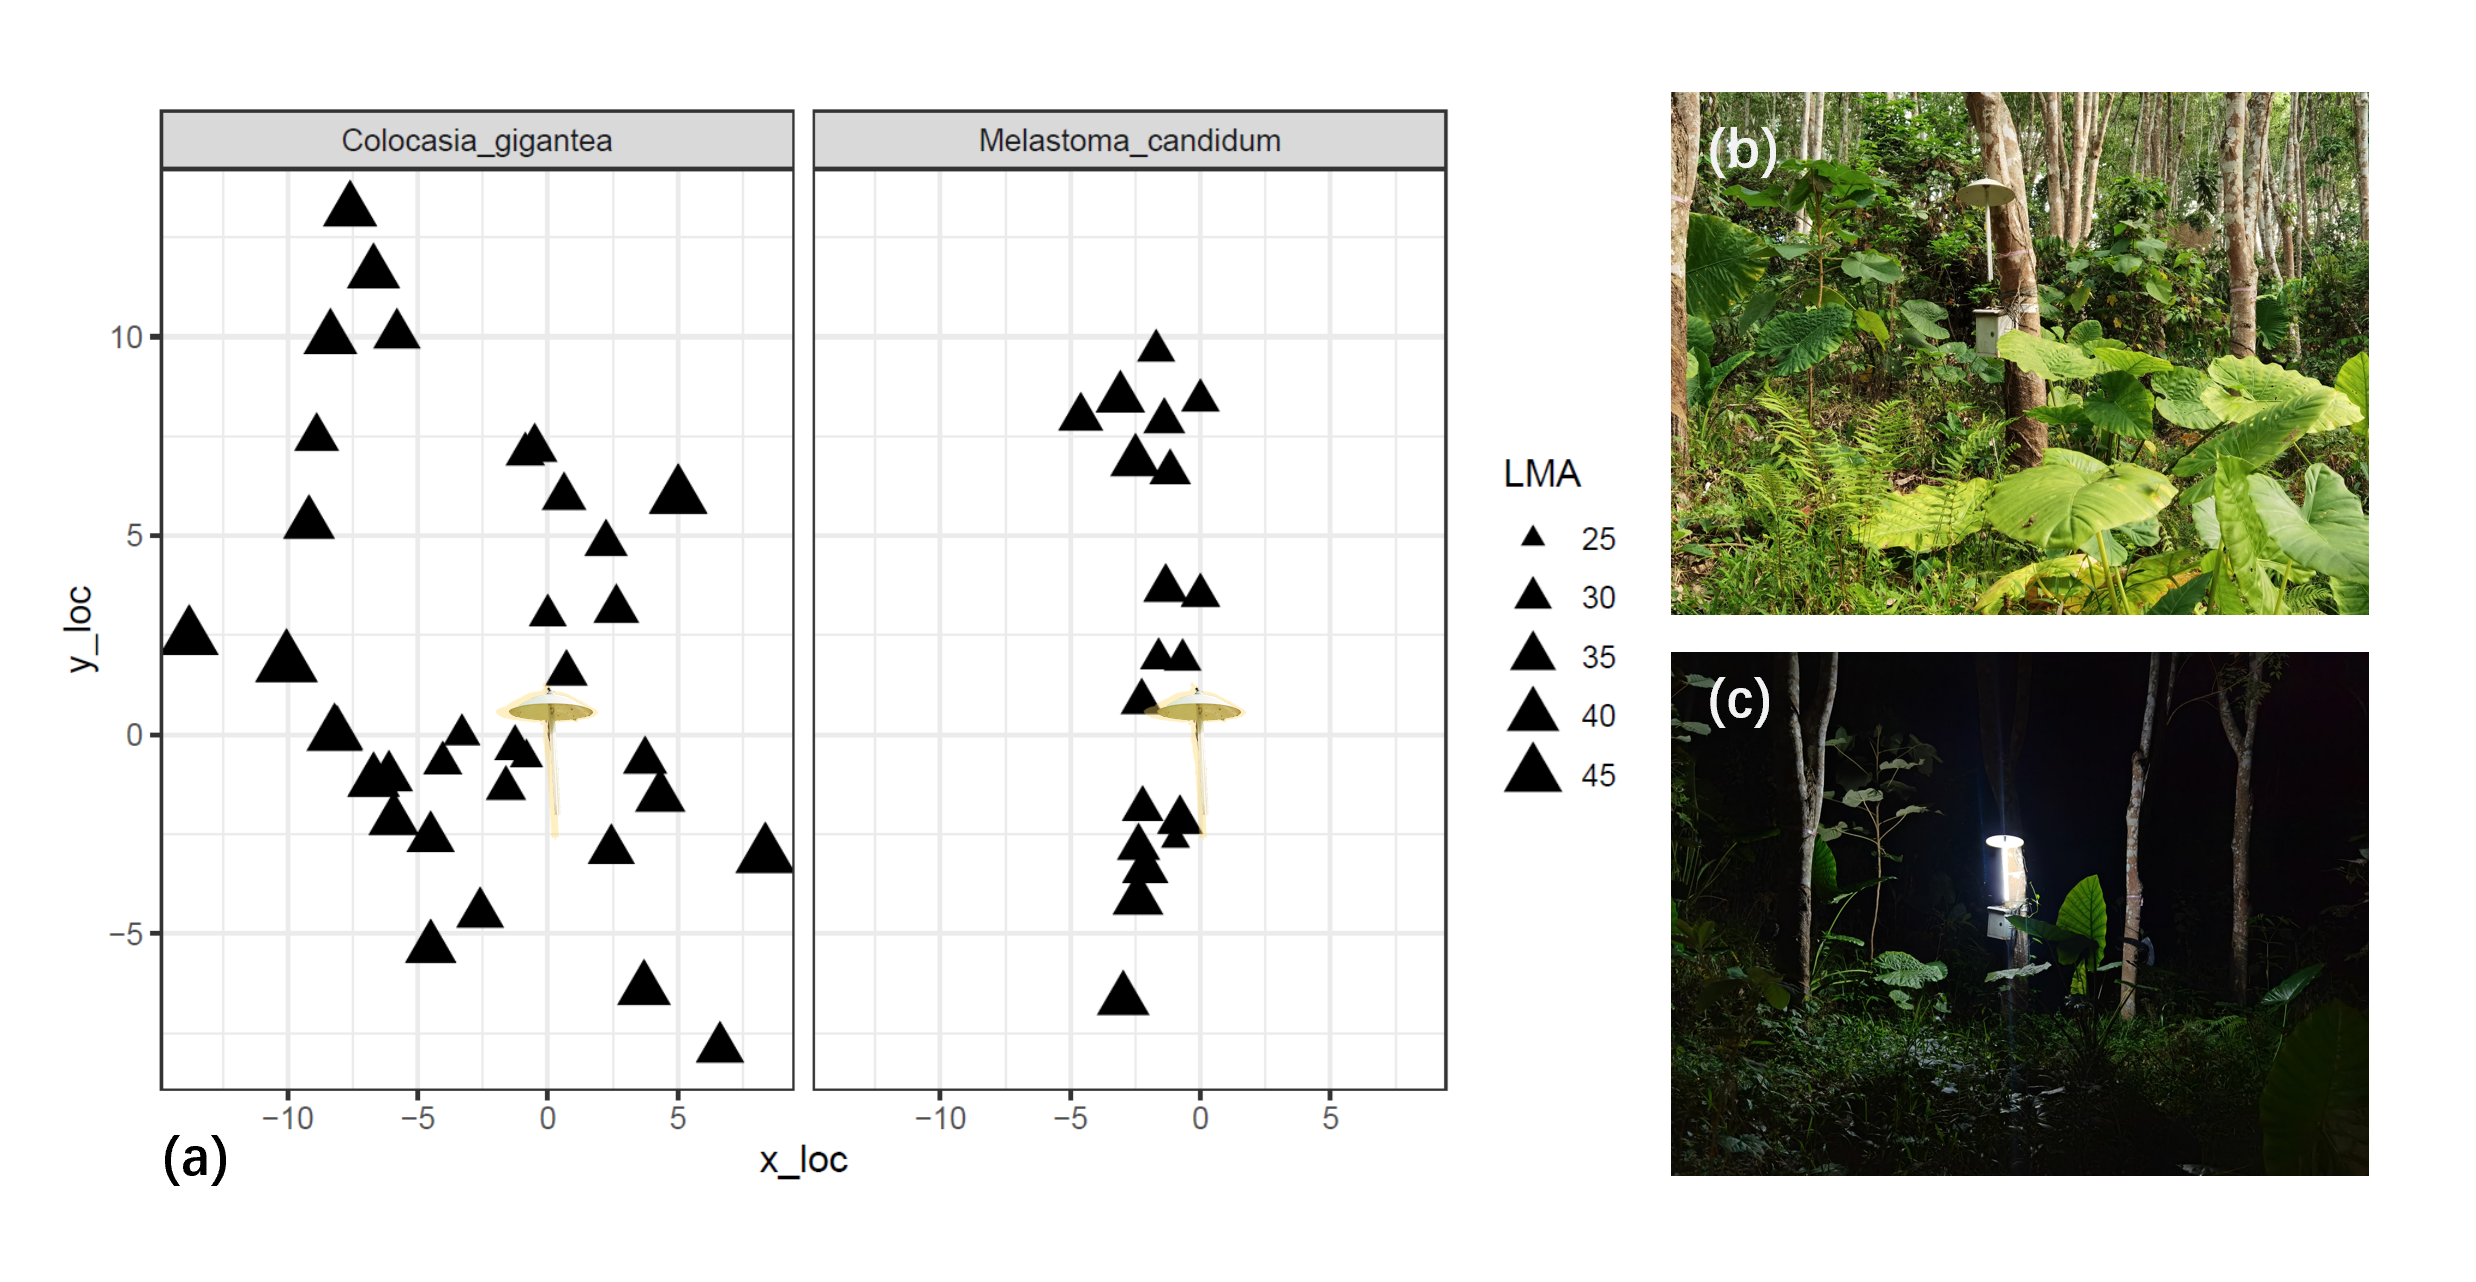
\includegraphics{../figs/LMA_distribution}

\newpage

\begin{table}

\caption{\label{tab:table}Coefficients table}
\centering
\begin{tabular}[t]{r|l|r|>{}l}
\hline
X & Parameters & mean\_value & quantile\_interval\\
\hline
\multicolumn{4}{l}{\textbf{Melastoma\_candidum}}\\
\hline
\hspace{1em}1 & ALAN's effect & -0.0422 & [-0.1129, 0.0276]\\
\hline
\hspace{1em}2 & Daylight's effect & -0.0006 & [-0.0761, 0.0744]\\
\hline
\hspace{1em}3 & interaction & -0.0308 & [-0.0836, 0.0216]\\
\hline
\multicolumn{4}{l}{\textbf{Colocasia\_gigantea}}\\
\hline
\hspace{1em}4 & ALAN's effect & -0.1043 & \textbf{[-0.1458, -0.0621]}\\
\hline
\hspace{1em}5 & Daylight's effect & 0.0495 & \textbf{[0.0051, 0.0938]}\\
\hline
\hspace{1em}6 & interaction & -0.0120 & [-0.0428, 0.0195]\\
\hline
\end{tabular}
\end{table}

\textbf{Table. 1.}\\
Results of Bayesian general linear mixed-effect models testing the
effects of artificial light at night, daylight and interaction on
experimental species. Significant effects (p \textless{} 0.05) are in
bold.

\newpage

\end{document}
